\section{评估}

为系统性评估 \SysName{}，我们围绕以下研究问题组织实验：

\noindent \textbf{Q1：} 在离线批量 Agent 推理中，\SysName{} 可以带来多大的端到端吞吐提升？（\S\ref{subsec:evalrq1}）

\noindent \textbf{Q2：} 在高并发下，\SysName{} 会如何影响 KV 缓存行为，尤其是缓存命中率与内存利用情况？（\S\ref{subsec:evalrq2}）

\noindent \textbf{Q3：} 固定大小的准入控制策略是否足以支持 Agent 工作负载？（\S\ref{subsec:evalrq3}）

\begin{table*}[t]
\caption{在不断升高的有效并发度下，离线 Agent 推理的端到端时延与加速比，单位为秒。}
\centering
\small
\begin{tabular}{l l c c c c}
\toprule
\textbf{模型} & \textbf{Batch / TP / \#GPU}
& \textbf{SGLang (s)}
& \textbf{SGLang + Request Control (s)}
& \textbf{SGLang + HiCache (s)}
& \textbf{\SysName{} (s)}\\
\midrule
& 256 / 8 / 8
& 1480 (1.00$\times$)
& 2049 (0.72$\times$)
& 976 (1.52$\times$)
& \textbf{362 (4.09$\times$)} \\

Qwen3-32B & 256 / 4 / 4
& 2213 (1.00$\times$)
& 1089 (2.03$\times$)
& 1678 (1.32$\times$)
& \textbf{757 (2.92$\times$)} \\

& 256 / 2 / 2
& 2527 (1.00$\times$)
& 1383 (1.83$\times$)
& 1112 (2.27$\times$)
& \textbf{846 (2.99$\times$)} \\

\midrule
& 16 / 16 / 16
& 873 (1.00$\times$)
& 861 (1.01$\times$)
& 2559 (0.34$\times$)
& \textbf{521 (1.68$\times$)} \\

DeepSeek-V3
& 32 / 16 / 16
& 1226 (1.00$\times$)
& 1367 (0.90$\times$)
& 2277 (0.54$\times$)
& \textbf{1018 (1.20$\times$)} \\

& 40 / 16 / 16
& 3877 (1.00$\times$)
& 2903 (1.34$\times$)
& 2320 (1.67$\times$)
& \textbf{2043 (1.90$\times$)} \\

\bottomrule
\end{tabular}

\label{tab:end_to_end_latency}
\end{table*}

\begin{table}[t]
\caption{DeepSeek-V3 在 TP=8、8 张 GPU 条件下，不同 batch 与并发配置对应的 KV 缓存命中率（\%）。\SysName{} 相比基线保持了更高命中率。}
\centering
\footnotesize
\label{tab:kv_hit_rate}
\begin{tabular}{>{\centering\arraybackslash}p{0.8cm}
                >{\centering\arraybackslash}p{1.2cm}
                >{\centering\arraybackslash}p{1.5cm}
                >{\centering\arraybackslash}p{1.8cm}
                >{\centering\arraybackslash}p{1.2cm}}
\toprule
Batch  & SGLang (\%) & SGLang + HiCache (\%) & SGLang + Request Control (\%) & \SysName{} (\%) \\
\midrule
16 & 80.38 & 97.48 & 69.00 & 96.38 \\
32 & 77.72 & 97.13 & 68.39 & 93.65 \\
40 & 35.41 & 96.08 & 32.21 & 73.36 \\
\bottomrule
\end{tabular}
\end{table}

\subsection{端到端性能}
\label{subsec:evalrq1}
为回答 Q1，我们评估了不同并发水平下离线批量 Agent 推理的端到端时延。对比对象包括三类基线：(i) \textbf{SGLang}，采用请求级 batching 与基于 LRU 的 KV 缓存淘汰；(ii) \textbf{带请求级准入控制的 SGLang}，通过固定请求上限限制并发；(iii) \textbf{带 HiCache 的 SGLang}，这是一种优先保留 KV 缓存并依赖 CPU 卸载的缓存中心方案。所有系统使用相同模型权重、提示词与 rollout 工作负载。实验平台为 NVIDIA H100 GPU（80GB），节点内通过 900 GB/s NVLink 互联，跨节点通过 8 路 400 Gbps RoCE 互联；软件栈包含 PyTorch 2.7.1、Python 3.12 与 CUDA 12.6。

\noindent\textbf{超参数设置。}
在我们的实现中，所有实验都使用统一控制参数。遵循 AIMD 拥塞控制的常见经验，我们将加性增大因子设为 $\alpha = 2$，乘性减小因子设为 $\beta = 0.5$，以在稳定探测容量与快速拥塞恢复之间取得平衡。利用率与命中率阈值设置为 $U_{low} = 0.2$、$U_{high} = 0.5$ 和 $H_{thresh} = 0.2$。附录~\ref{appendix:sensitivity} 给出了利用率阈值的敏感性分析。结果表明，$U_{high}$ 可以在较宽且不敏感的区间（0.5--0.6）内选择，而 $U_{low}$ 则需要更谨慎地校准，因为它直接决定窗口增长的激进程度。我们最终采用的 $U_{low} = 0.2$ 和 $U_{high} = 0.5$ 在主动探测容量与及时响应拥塞之间取得了较好平衡。

我们在两类代表性大模型 Qwen3-32B 与 DeepSeek-V3 上报告端到端批量时延，并通过 batch size 与张量并行（TP）控制有效并发。时延越低，代表离线 Agent 推理的有效吞吐越高。表~\ref{tab:end_to_end_latency} 总结了所有配置下的结果。

\SysName{} 在两类模型与所有并发配置上都取得了最低时延，并且在高并发场景下优势尤其明显。对于 Qwen3-32B，相比原生 SGLang，\SysName{} 的时延最高可降低 $4.09\times$；相比请求级准入控制，最高可降低接近 $3\times$。随着 TP 减小、每张 GPU 的有效并发提高，基线系统会遭遇明显放缓，而 \SysName{} 的优势继续扩大。对于 DeepSeek-V3，\SysName{} 在大 batch 下同样优于全部基线，并避免了 SGLang 与缓存中心方案中常见的时延膨胀。

请求中心和缓存中心基线之所以表现不佳，是因为它们无法让调度决策与 Agent 级内存局部性对齐。请求级准入控制看不到长期运行 Agent 所积累的 KV 工作集，因此常常在其缓存状态已经被淘汰之后才安排其继续执行，导致反复重计算。缓存中心方案（如 HiCache）虽然能通过 CPU 卸载降低重计算频率，但在高并发条件下，PCIe 竞争与排队时延会成为主导，从而限制其效果。

与之相对，\SysName{} 在 Agent 粒度上调节并发，直接限制活跃 Agent 的整体 KV 工作集规模。这种方式能在执行中期阻止过量准入，维持较高缓存命中率，并在整个推理过程中保持稳定的批处理效率。因此，\SysName{} 才能在不同模型与 batch 配置上持续保持低时延。

\begin{figure}[tb]
    \centering
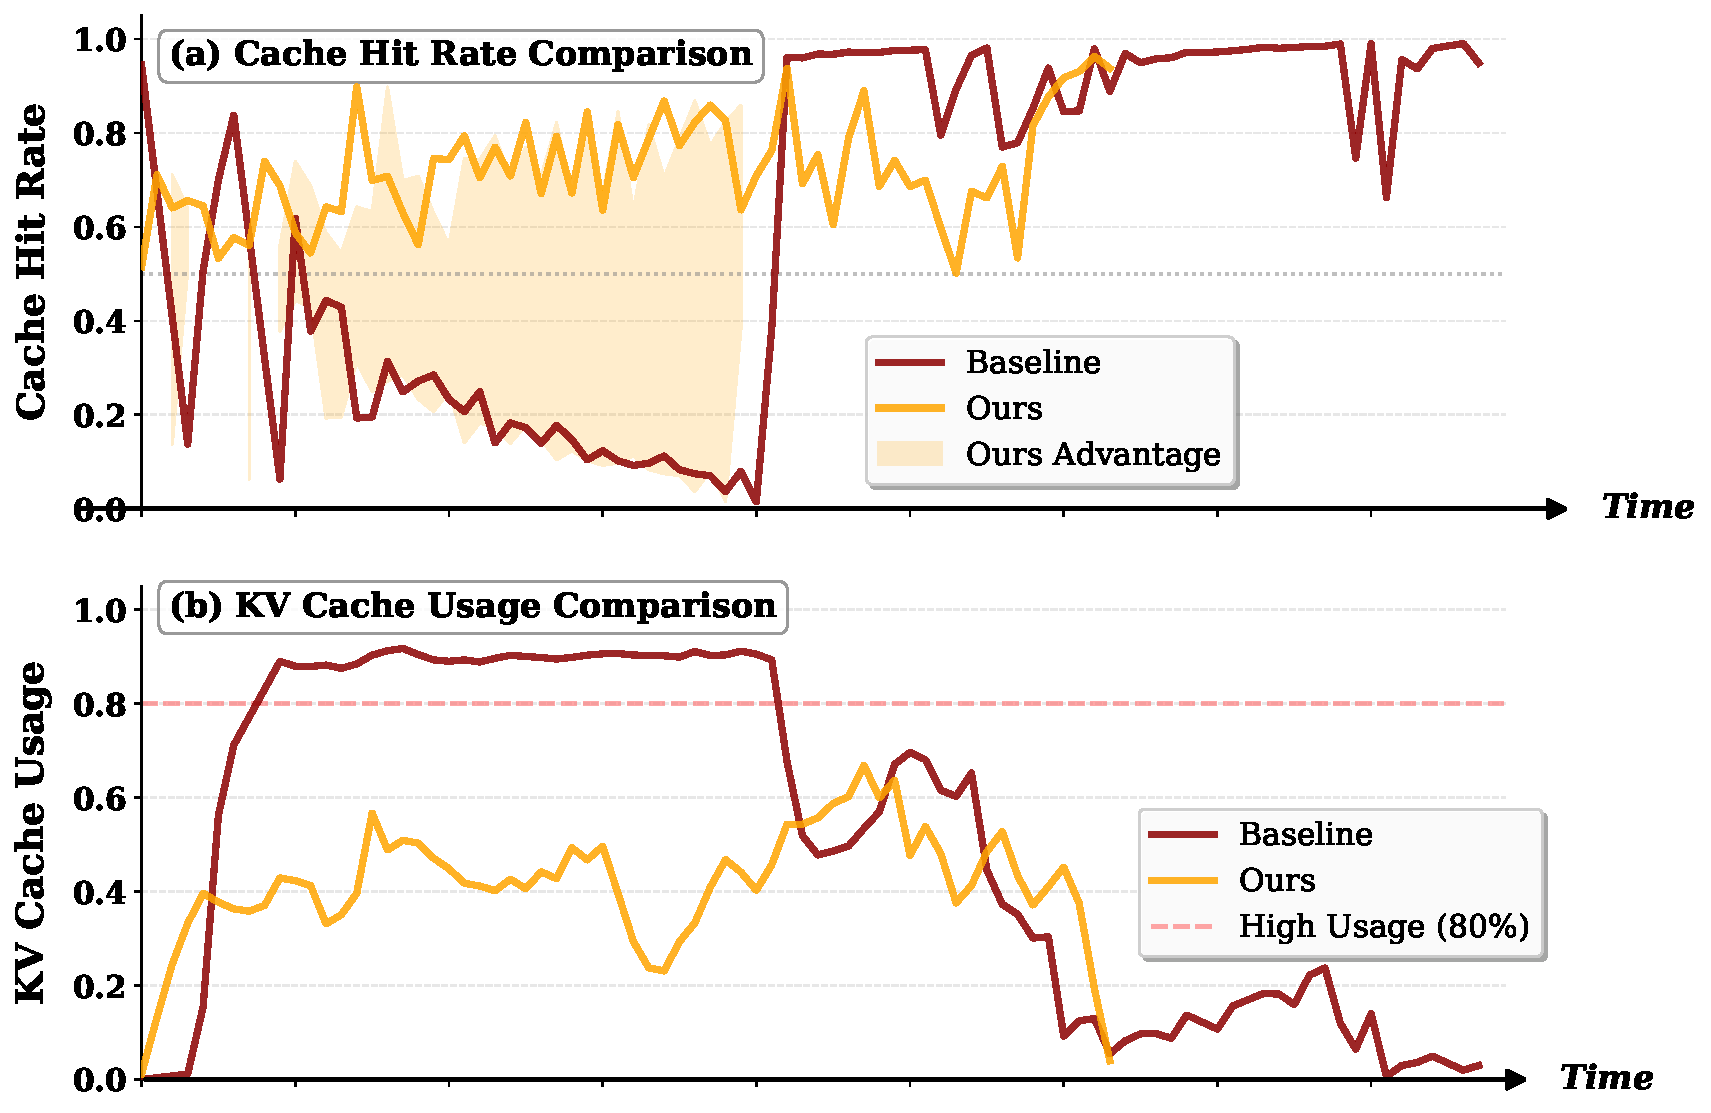
\includegraphics[width=0.98\linewidth]{figure/dual_kv_cache_comparison.pdf}
    \caption{Qwen3-32B 在受限资源条件下（Batch 256、TP=2、2 张 GPU）进行大批量离线 Agent 推理时，KV 缓存的时间动态。}
    \label{fig:kv_time_series}
\end{figure}

\subsection{KV 缓存行为分析}
\label{subsec:evalrq2}
表~\ref{tab:kv_hit_rate} 报告了与 \S\ref{subsec:evalrq1} 相同配置下，DeepSeek-V3 的平均 KV 缓存命中率。结果与此前观察到的端到端时延趋势高度一致，并直接为中期抖动提供了证据。

随着并发提升，SGLang 的 KV 缓存命中率迅速下降。小 batch 下命中率尚可，但在 batch 为 40 的配置下会骤降到 $35.41\%$。即使通过请求级准入限制飞行中的请求数量，请求级控制基线在高并发下的命中率仍会降到 $32.21\%$。HiCache 通过积极保留 KV 缓存并卸载到 CPU，在所有配置下都保持了很高命中率；但如 \S\ref{subsec:evalrq1} 所示，仅有高命中率并不足以保证低时延，因为 PCIe 传输本身的额外开销会抵消这一优势。

相比之下，\SysName{} 在避免过度卸载的同时仍保持了较高 KV 缓存命中率。由于它在 Agent 粒度上控制并发，能够在抖动阶段保留更好的 KV 局部性，同时避免显存过量承诺。这种平衡正是其在 Q1 中实现最低时延并显著优于 SGLang 与请求级基线的原因。

为了更细致地理解时间动态，图~\ref{fig:kv_time_series} 给出了 batch size 为 256 时 Agent 推理全过程中的 KV 缓存命中率（上）与使用率（下）。当多个 Agent 同步推进到中等长度步骤时，KV 缓存使用率接近容量上限（约 80\%），而基线方法的命中率会急剧下降。\SysName{} 通过调节 Agent 准入维持明显更高的命中率，从而避免多个 Agent 同时对 KV 缓存槽造成过量承诺。

\subsection{静态准入控制与缓存感知准入控制}
\label{subsec:evalrq3}
为回答 Q3，我们评估固定大小的准入控制是否足以支撑 Agent 工作负载。实验中我们测试了多个固定准入水平（30、32、64、128），并与自适应策略 \SysName{} 对比。

图~\ref{fig:e2ecache} 给出了结果。较小的固定水平（如 30--64）相比完全不控的基线能够降低时延，但往往过于保守，会在某些执行阶段低估可用 GPU 资源。较大的固定水平（如 128）则允许更多并发，却会导致显存过量承诺，引发 KV 缓存抖动并推高时延。\SysName{} 取得了最低观测时延 846 ms，相比最佳固定水平配置可进一步提升约 $1.5$--$2.9\times$，相对无控制基线提升 $2.99\times$。

总的来说，静态准入控制是一种脆弱策略：要么浪费 GPU 资源，要么触发 KV 缓存抖动，其表现高度依赖具体阈值选择。相比之下，\SysName{} 通过阶段感知的并发调节，在 Agent 工作负载中同时实现了高吞吐与稳定执行，而这正是固定大小控制难以做到的。

\begin{figure}[tb]
    \centering
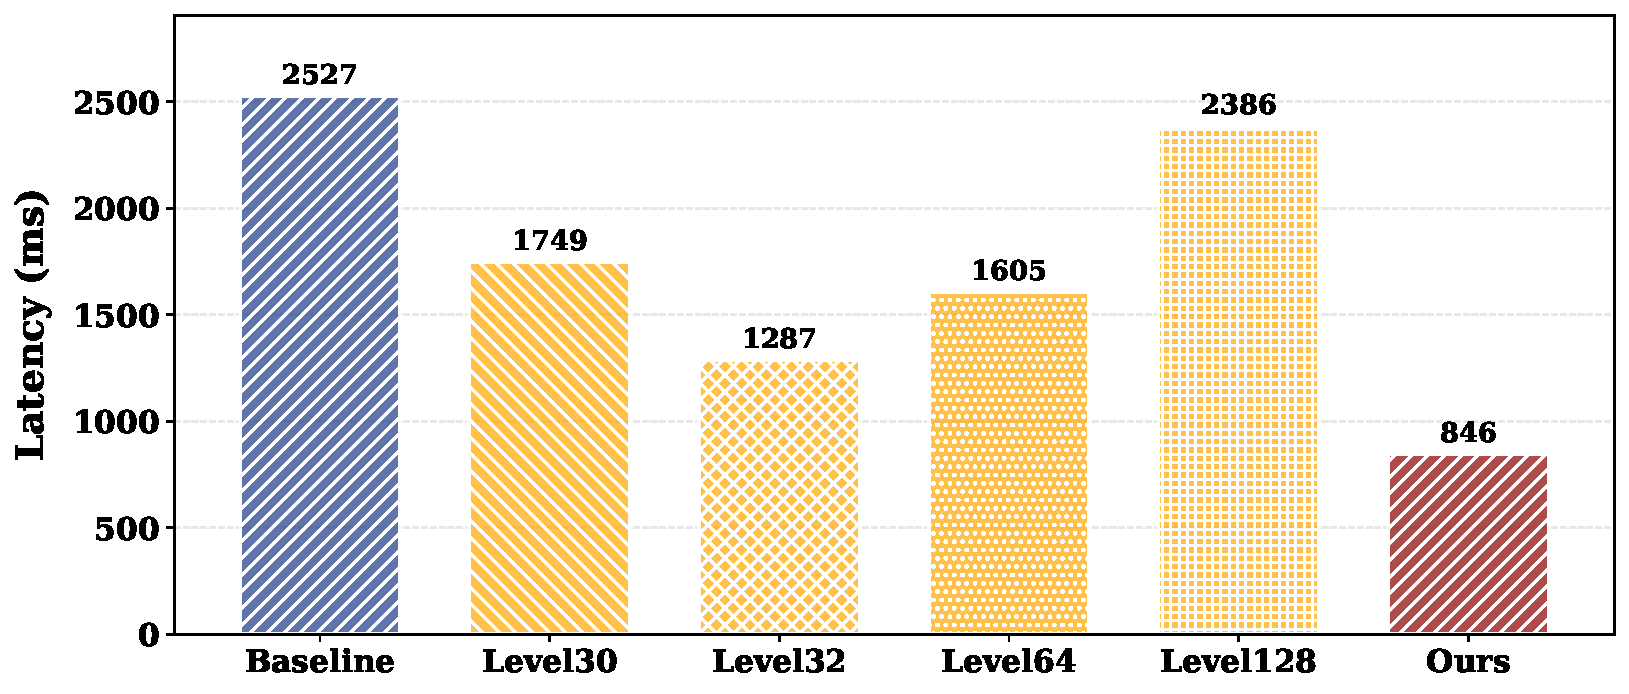
\includegraphics[width=0.98\linewidth]{figure/admission_levels_comparison.pdf}
    \caption{Qwen3-32B（Batch 256、TP 2、2 张 GPU）在固定准入控制与自适应准入控制下的端到端时延对比。}
    \label{fig:e2ecache}
\end{figure}
